\section*{CHƯƠNG 3: MCU VÀ PHẦN CỨNG ĐƯỢC SỬ DỤNG TRONG THỰC TẬP}
\addcontentsline{toc}{section}{\numberline {} CHƯƠNG 3: MCU VÀ PHẦN CỨNG ĐƯỢC SỬ DỤNG TRONG THỰC TẬP}
\setcounter{section}{3}
\setcounter{figure}{0}
\setcounter{subsection}{0}
\subsection{ARDUINO NANO CH340}
\begin{figure}[H]
	\centering
	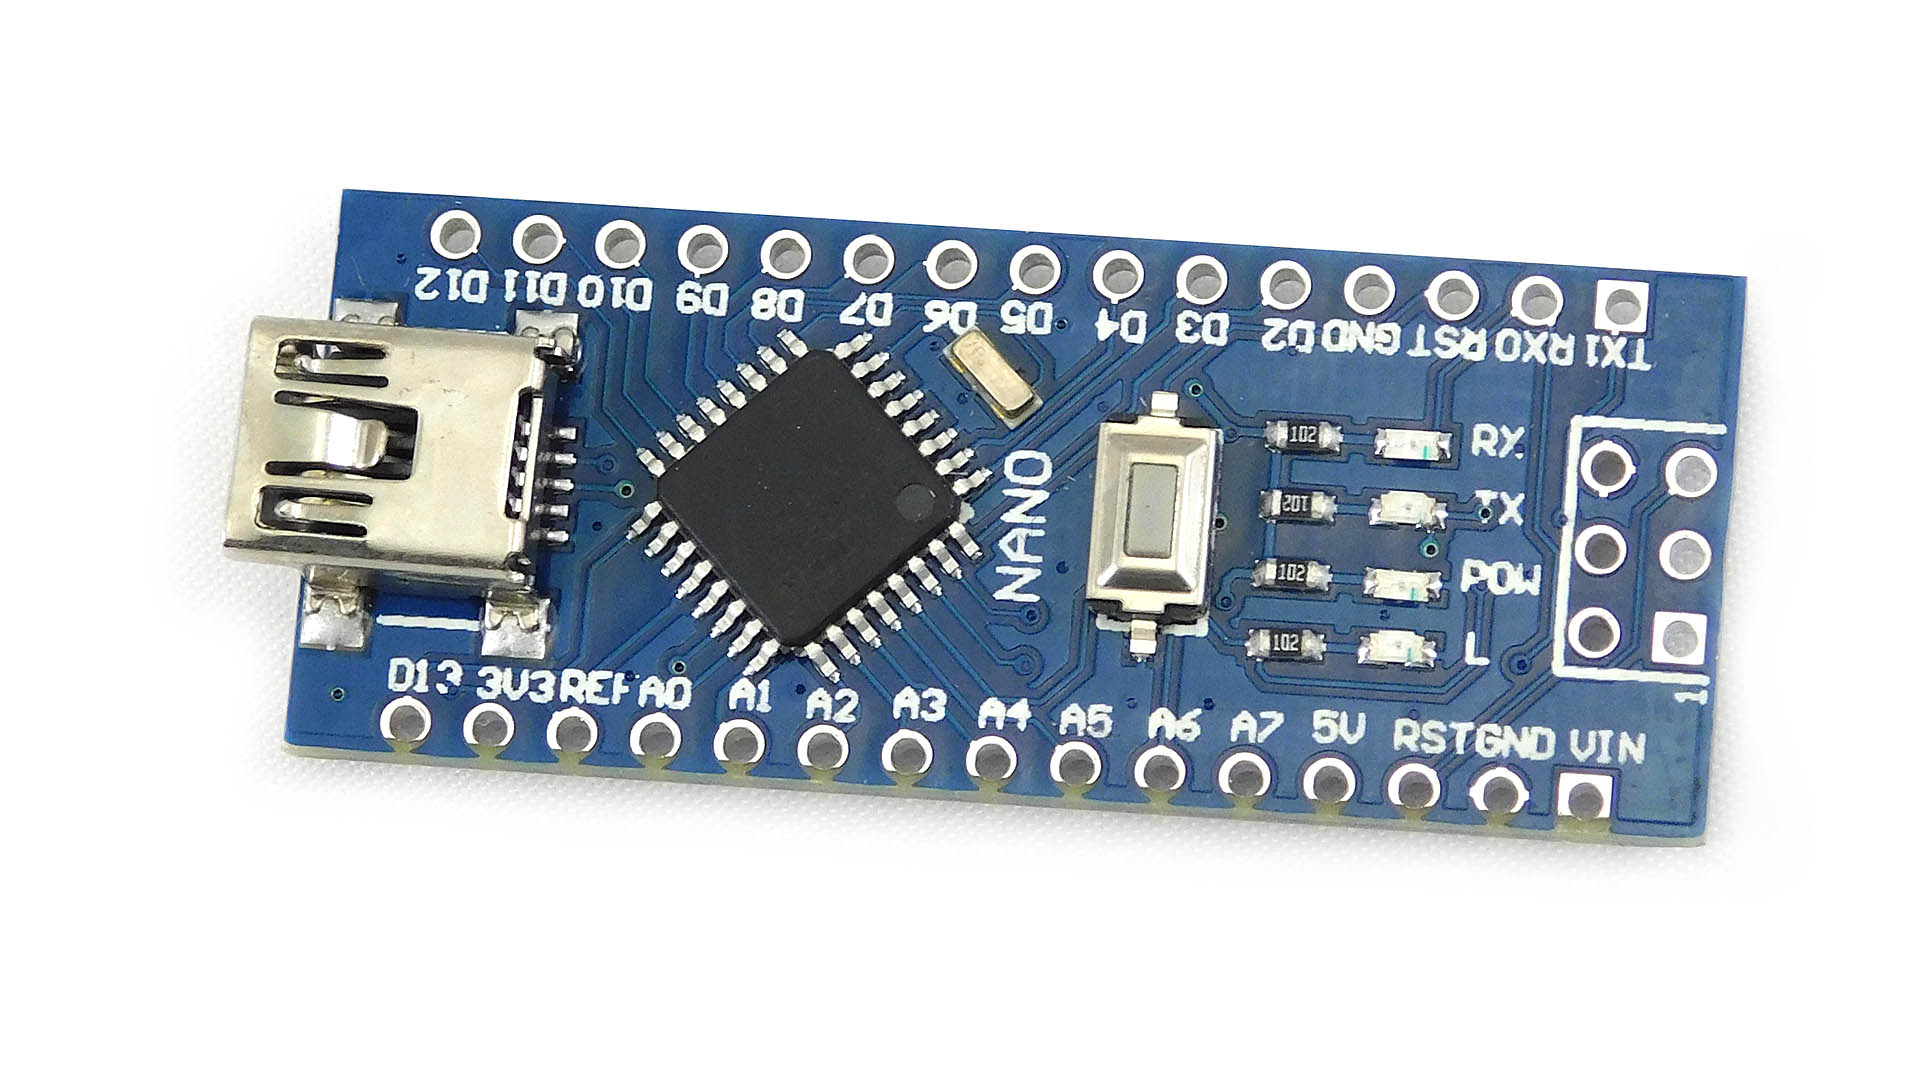
\includegraphics[scale=0.15]{Chapter 3/image chapter 3/nano.jpg}
	\caption[Arduino nano CH340]{Arduino nano CH340}
	\label{hinh31}
\end{figure}
Mạch Arduino Nano CH340 có kích thước nhỏ gọn, có thiết kế và chuẩn chân giao tiếp tương đương với Arduino Nano chính hãng, tuy nhiên mạch sử dụng chip nạp chương trình và giao tiếp UART CH340 giá rẻ để tiết kiệm chi phí.\\
\indent Arduino Nano là phiên bản nhỏ gọn của Arduino Uno R3 sử dụng MCU ATmega328P-AU dán, vì cùng MCU nên mọi tính năng hay chương trình chạy trên Arduino Uno đều có thể sử dụng trên Arduino Nano, một ưu điểm của Arduino Nano là vì sử dụng phiên bản IC dán nên sẽ có thêm 2 chân Analog A6, A7 so với Arduino Uno.\\
\begin{figure}[H]
	\centering
	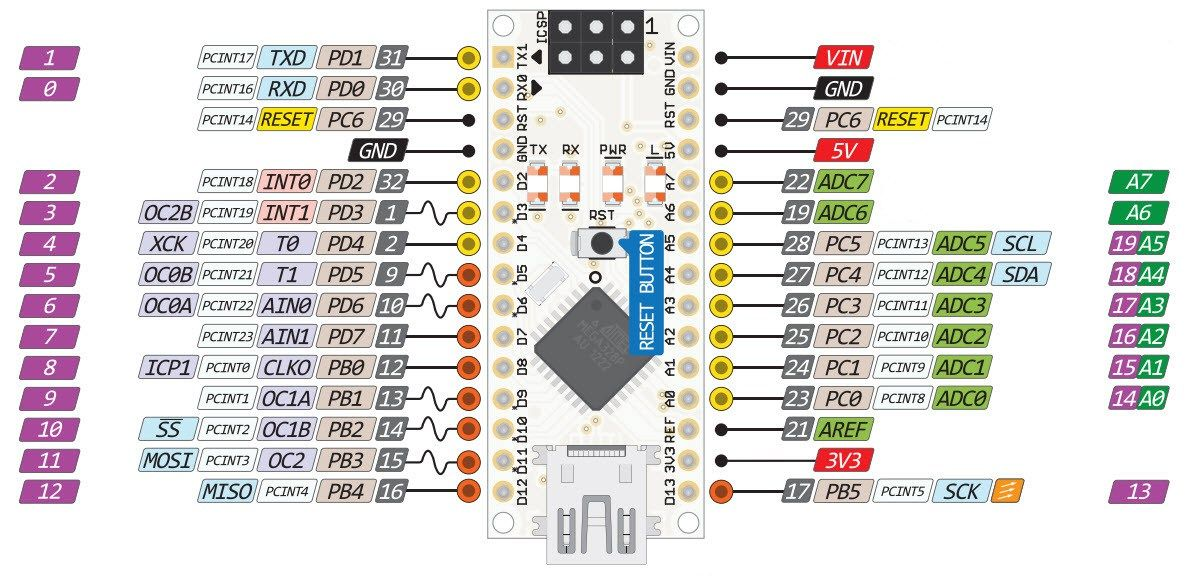
\includegraphics[scale=.7]{Chapter 3/image chapter 3/sodoNano.png}
	\caption[Sơ đồ chân của Arduino nano CH340]{Sơ đồ chân của Arduino nano CH340}
	\label{hinh32}
\end{figure}
\indent \textbf{Thông số kỹ thuật:}\\
\begin{itemize}
	\item Thiết kế theo đúng chuẩn chân, kích thước của Arduino Nano chính hãng.
	\item IC chính: ATmega328P-AU.
	\item IC nạp và giao tiếp UART: CH340.
	\item Điện áp cấp: 5VDC cổng USB hoặc 6-9VDC chân Raw.
	\item Mức điện áp giao tiếp GPIO: TTL 5VDC.
	\item Dòng GPIO: 40mA.
	\item Số chân Digital: 14 chân, trong đó có 6 chân PWM.
	\item Số chân Analog: 8 chân (hơn Arduino Uno 2 chân).
	\item Flash Memory: 32KB (2KB Bootloader).
	\item SRAM: 2KB
	\item EEPROM: 1KB
	\item Clock Speed: 16Mhz.
	\item Tích hợp Led báo nguồn, led chân D13, LED RX, TX.
	\item Tích hợp IC chuyển điện áp 5V LM1117.
	\item Kích thước: 18.542 x 43.18mm
\end{itemize}
\subsection{RASPBERRY PI 3 MODEL B+}
\begin{figure}[H]
	\centering
	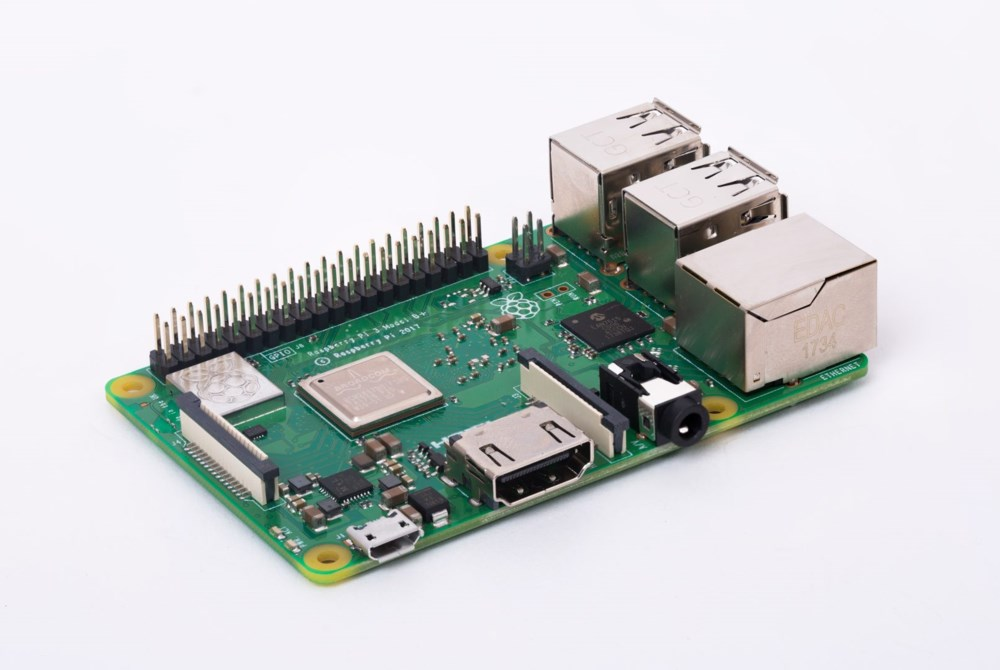
\includegraphics[scale=.5]{Chapter 3/image chapter 3/rasp3.jpg}
	\caption[Raspberry Pi 3 Model B+ ]{Raspberry Pi 3 Model B+}
	\label{hinh33}
\end{figure}
Raspberry Pi 3 Model B+ là một phiên bản nâng cấp của Raspberry Pi 3 Model B đã từng ra mắt cách đây hơn 2 năm. Trước kia, thường khoảng 1 năm thì Raspberry Pi sẽ được nâng cấp 1 lần nhưng từ phiên bản 3 thì Raspberry Pi đã làm điều này chậm hơn một chút dù doanh số bán lên tới 14 triệu máy.\\
\indent Với thế hệ Raspberry Pi 3 mới nhất và mạnh nhất hiện nay trong dòng Raspberry Pi, bản nâng cấp vừa ra mắt hôm nay chủ yếu mang đến tốc độ nhanh hơn về mọi mặt.\\
\indent Cụ thể, điểm nâng cấp chính của Raspberry Pi 3 Model B+ là vi xử lý và kết nối mạng. Model B+ dùng vi xử lý Broadcom BCM2837B0 4 nhân 1.4GHz (cao hơn so với BCM2837 1.2GHz trên Pi 3 Model B).\\
\indent Với các công việc đòi hỏi tốc độ mạng nhanh, Pi 3 Model B+ có thể đáp ứng với kết nối Wi-Fi 2 băng tần 2.4GHz và 5GHz (dual band), Ethernet gigabit (qua cổng USB 2.0) tốc độ lên đến 300Mbps, gấp 3 lần so với Pi 3 Model B. Thiết bị cũng hỗ trợ Bluetooth 4.2 và Bluetooth LE giúp kết nối tốt hơn với các thiết bị thông minh khác.\\
\indent Cuối cùng, Model B+ còn có Power over Ethernet (PoE) giúp cung cấp nguồn điện cho thiết bị thông qua dây cắm Ethernet nhưng phải thông qua một HAT mở rộng.\\
\indent Ngoài những nâng cấp trên thì ngoại hình và kích thước Model B+ vẫn y hệt Model B nên hoàn toàn tương thích với mọi case và phụ kiện trước đây dành cho Model B. Cấu hình chi tiết Raspberry Pi 3 Model B+:
\begin{itemize}
	\item SoC: Broadcom BCM2837B0, Cortex-A53 (ARMv8) 64-bit SoC @ 1,4 GHz
	\item RAM: 1 GB LPDDR2 SDRAM
	\item Wi-Fi b/g/n/ac
	\item Bluetooth 4.2, BLE
	\item Gigabit Ethernet over USB 2.0 (maximum throughput 300 Mbps)
	\item 40-pin GPIO
	\item HDMI
	\item 4 x cổng USB 2.0
	\item Khe cắm thẻ Micro SD
	\item Hỗ trợ Power-over-Ethernet (PoE)
	\item Cải thiện PXE network và USB mass-storage booting
	\item Tản nhiệt tốt hơn Model B
\end{itemize}
\begin{figure}[H]
	\centering
	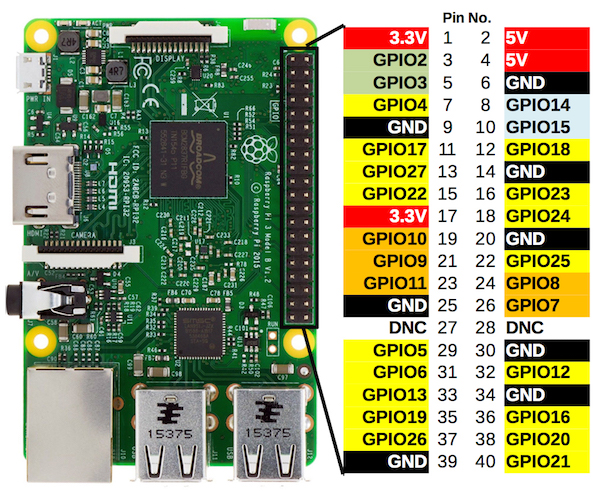
\includegraphics[scale=.5]{Chapter 3/image chapter 3/raspGPIO.jpg}
	\caption[Sơ đồ các chân GPIO của Raspberry Pi 3 Model B+]{Sơ đồ các chân GPIO của Raspberry Pi 3 Model B+}
	\label{hinh34}
\end{figure}
\subsection{MODULE RF UART E32-TTL-100}
\begin{figure}[H]
	\centering
	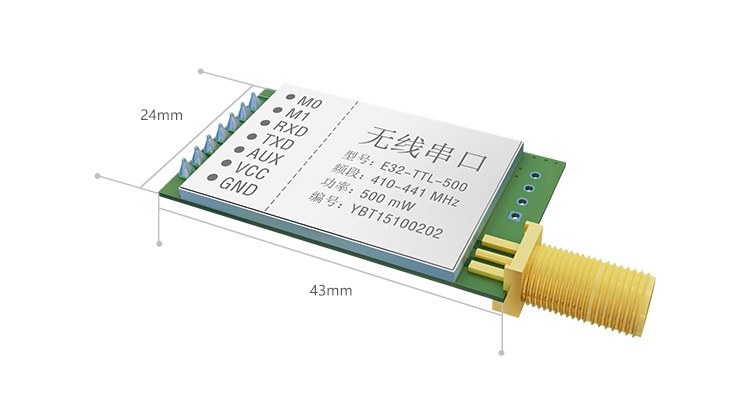
\includegraphics[scale=.4]{Chapter 2/image chapter 2/E32.jpg}
	\caption[Module RF UART E32-TTL-100]{Module RF UART E32-TTL-100}
	\label{hinh35}
\end{figure}
\begin{figure}[H]
	\centering
	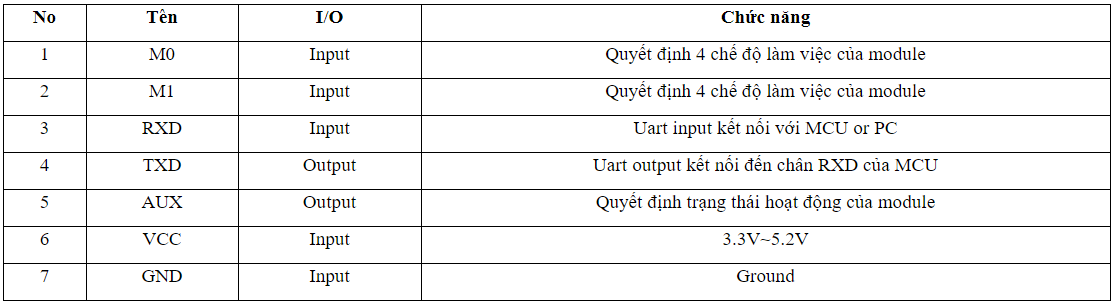
\includegraphics[scale=.5]{Chapter 2/image chapter 2/sodochanvachucnangE32.png}
	\caption[Sơ đồ chân và chức năng của module LoRa E32]{Sơ đồ chân và chức năng của module LoRa E32}
	\label{hinh36}
\end{figure}
Mạch thu phát RF UART Lora SX1278 433Mhz 3000m sử dụng chip SX1278 của nhà sản xuất SEMTECH chuẩn giao tiếp LORA (Long Range), chuẩn LORA mang đến hai yếu tố quan trọng là tiết kiệm năng lượng và khoảng cách phát siêu xa ( Ultimate long range wireless solution), ngoài ra nó còn có khả năng cấu hình để tạo thành mạng nên hiện tại được phát triển và sử dụng rất nhiều trong các nghiên cứu về IoT.\\
\indent Mạch thu phát RF UART Lora SX1278 433Mhz 3000m được tích hợp phần chuyển đổi giao tiếp SPI của SX1278 sang UART giúp việc giao tiếp và sử dụng rất dễ dàng, chỉ cần kết nối với Software của hãng để cấu hình địa chỉ , tốc độ và công suất truyền là có thể sử dụngnguyễn2000chu.\\
\indent \textbf{Thông số kỹ thuật:}
\begin{itemize}
	\item Model: E32-TTL-100 RF
	\item Điện áp hoạt đông: 2.3 - 5.5 VDC
	\item Điện áp giao tiếp: TTL-3.3V
	\item Giao tiếp UART Data bits 8, Stop bits 1, Parity none, tốc độ từ 1200 - 115200.
	\item Tần số: 410 - 441Mhz
	\item Công suất: 20dbm (100mW)
	\item Khoảng cách truyền tối đa trong điều kiện lý tưởng: 3000m
	\item Tốc độ truyền: 0.3 - 19.2 Kbps ( mặc định 2.4 Kbps)
	\item 512bytes bộ đệm
	\item Hỗ trợ 65536 địa chỉ cấu hình.
	\item Kích thước: 21x36mm.
\end{itemize}
\begin{figure}[H]
	\centering
	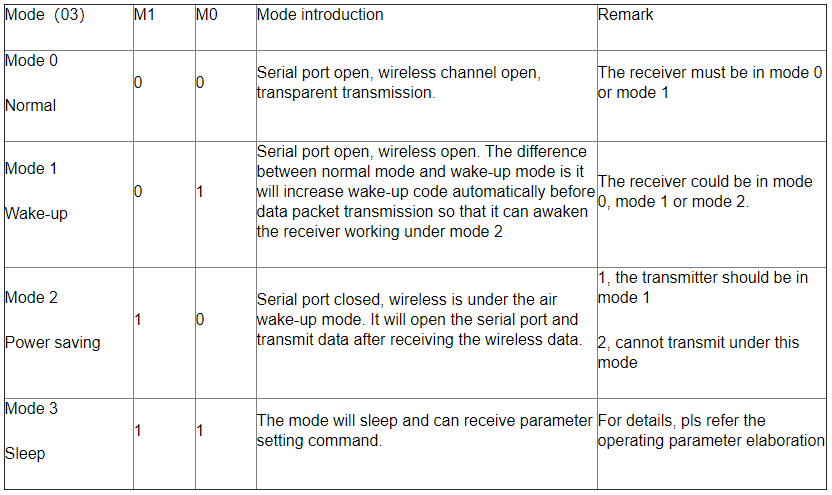
\includegraphics[scale=.5]{Chapter 2/image chapter 2/workmodeE32.png}
	\caption[Chế độ làm việc của module LoRa E32]{Chế độ làm việc của module LoRa E32}
	\label{hinh37}
\end{figure}
\subsection{DHT22 TEMPERATURE AND HUMIDITY SENSOR}
\begin{figure}[H]
	\centering
	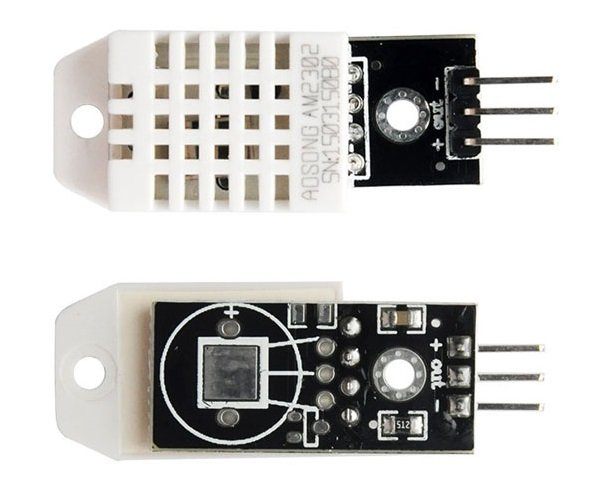
\includegraphics[scale=.5]{Chapter 3/image chapter 3/DHT22.jpg}
	\caption[Module DHT22]{Module DHT22}
	\label{hinh38}
\end{figure}
Cảm biến độ ẩm, nhiệt độ DHT22 Temperature Humidity Sensor ra chân là phiên bản ra chuẩn chân cắm thông dụng 2.54mm hàn sẵn trên mặt in với trở kéo dễ dàng sử dụng, ứng ụng đo độ ẩm, nhiệt độ môi trường với độ chính xác cao, cảm biến có chất lượng tốt, độ bền và độ ổn định cao.\\
\indent \textbf{Thông số kỹ thuật:}
\begin{itemize}
	\item Nguồn sử dụng: 3~5 VDC.
	\item Dòng sử dụng: 2.5mA max (khi truyền dữ liệu).
	\item Đo tốt ở độ ẩm 0100%RH với sai số 2-5%.
	\item Đo tốt ở nhiệt độ -40 to 80°C sai số ±0.5°C.
	\item Tần số lấy mẫu tối đa 0.5Hz (2 giây 1 lần)
	\item Kích thước 27mm x 59mm x 13.5mm (1.05" x 2.32" x 0.53")
	\item Chân tín hiệu: 5VDC(+) | OUT | GND (-) (chân out nối trực tiếp với chân giao tiếp của VĐK không cần trở kéo vì đã có sẵn trên mạch).
\end{itemize}
\subsection{MODULE 2 RELAY OPTO 5VDC}
\begin{figure}[H]
	\centering
	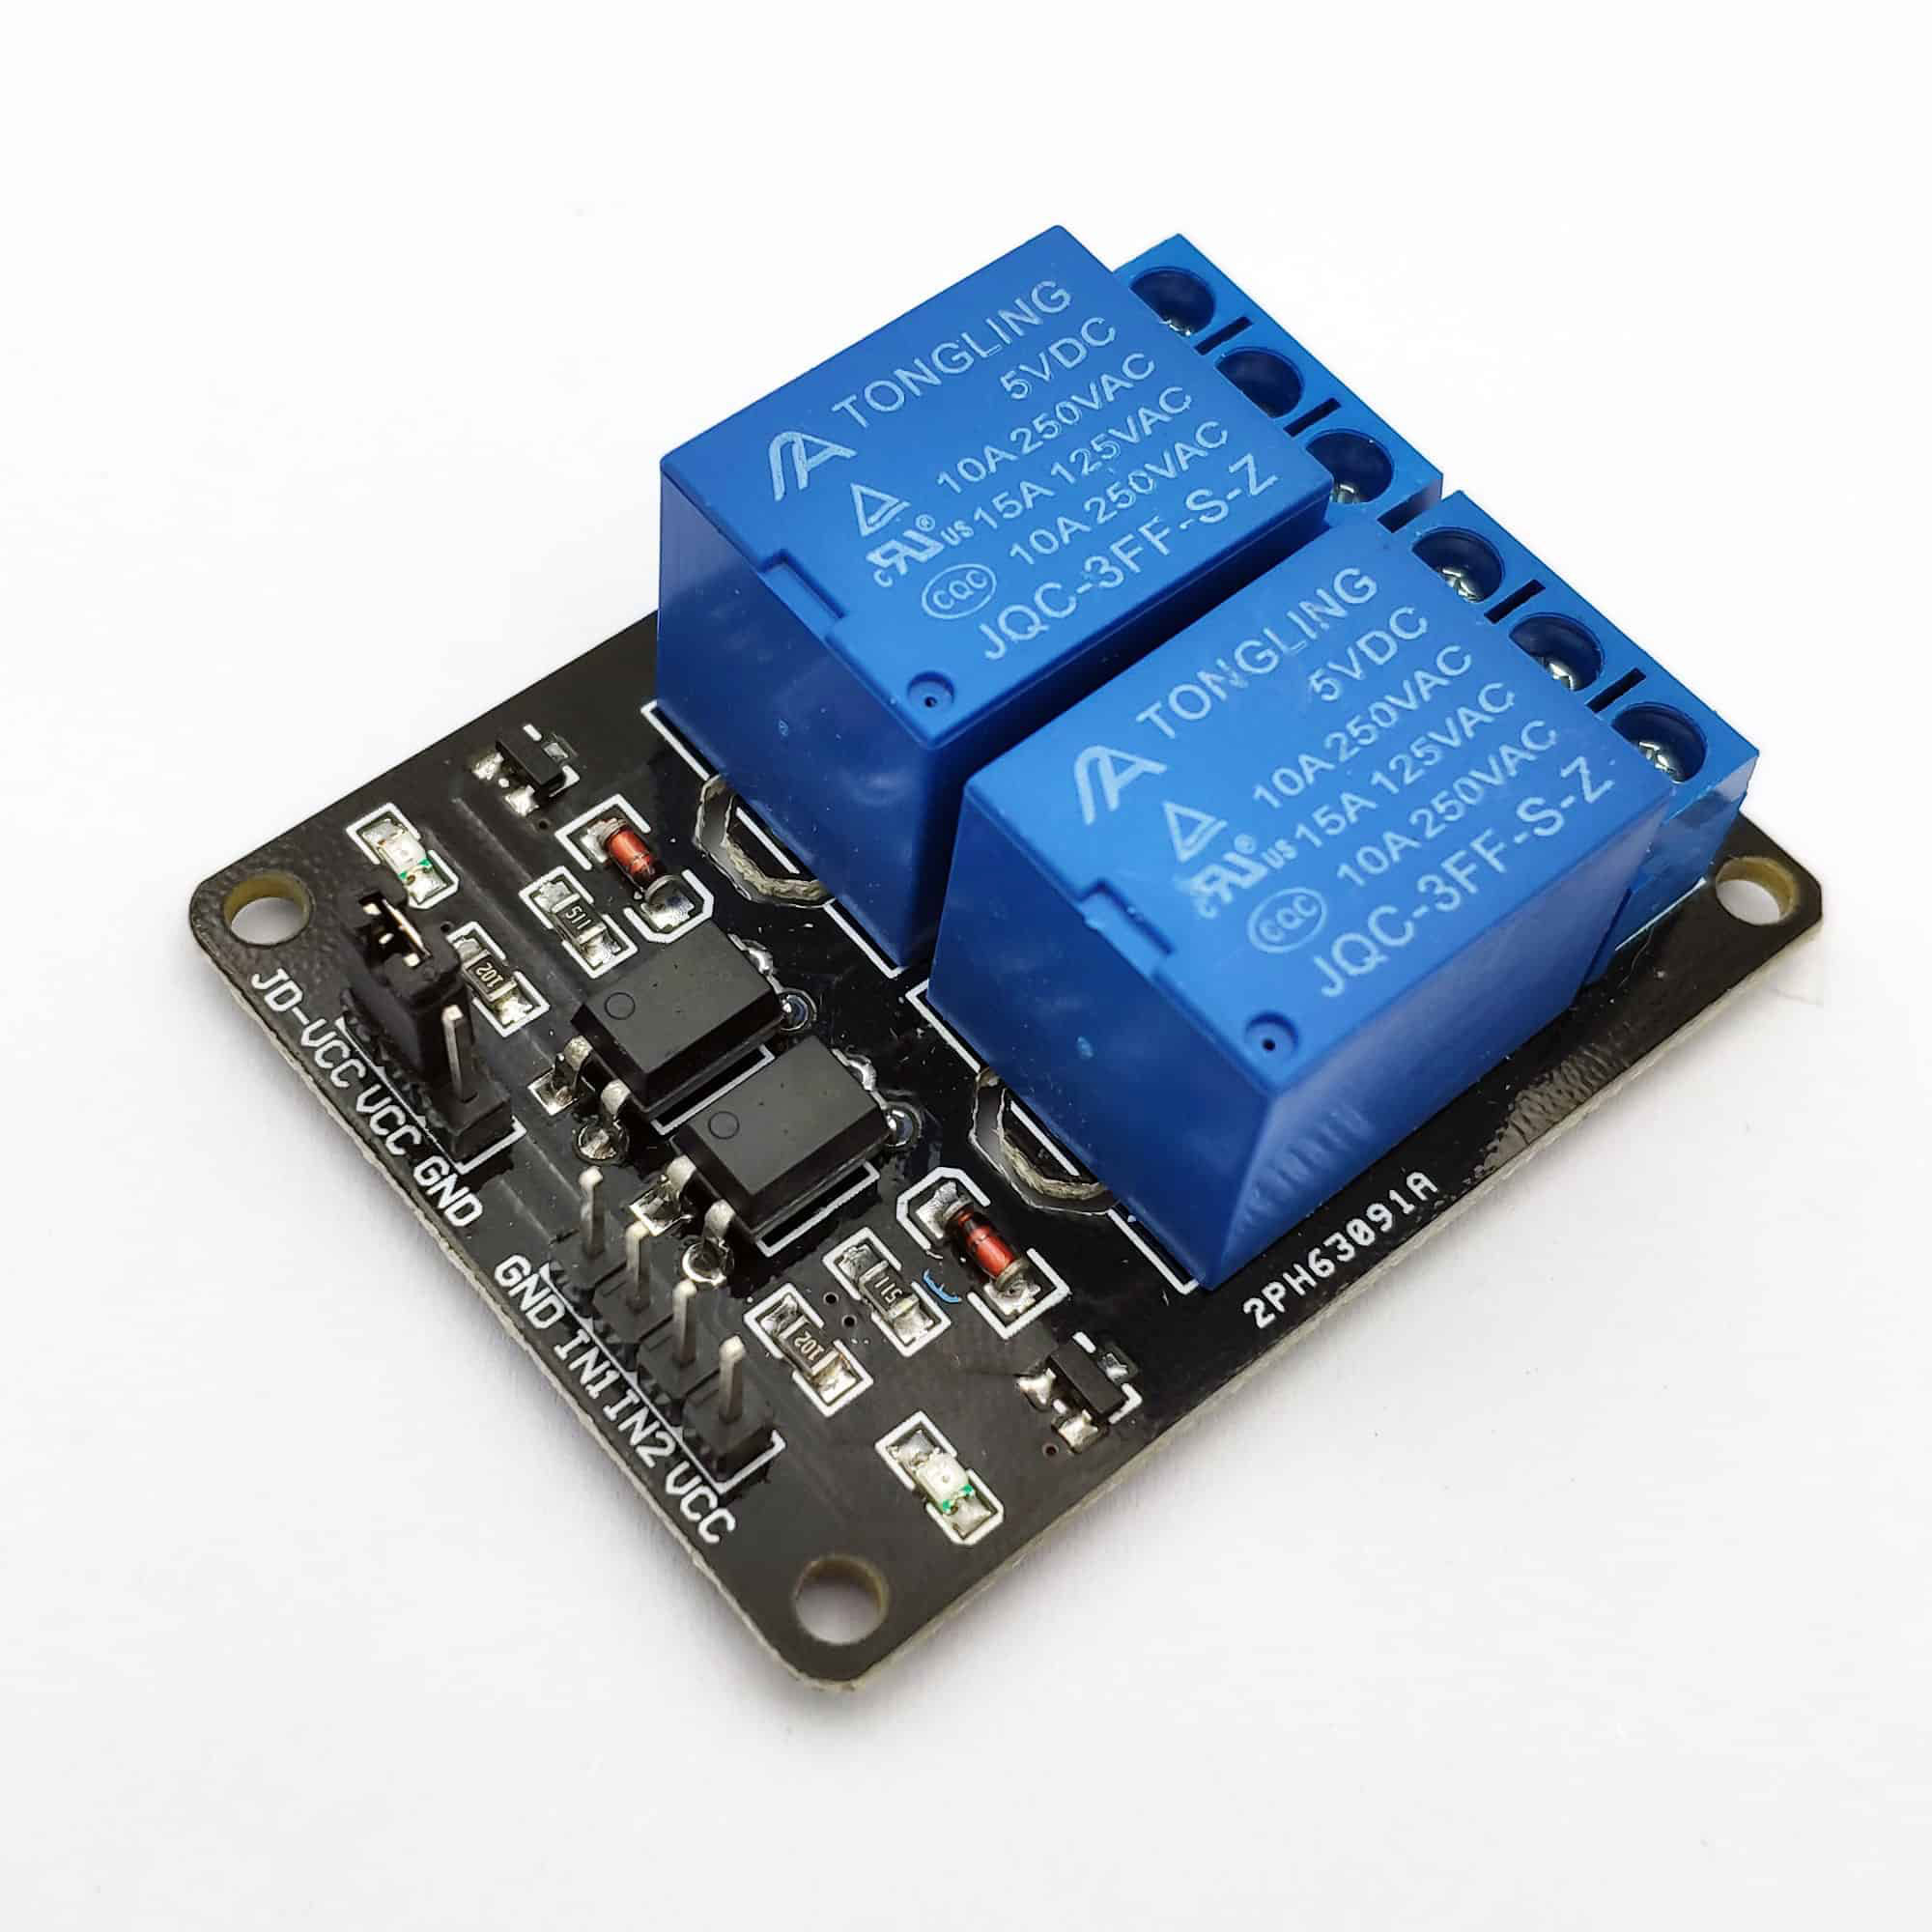
\includegraphics[scale=.1]{Chapter 3/image chapter 3/2relay.jpg}
	\caption[Module 2 relay opto 5VDC]{Module 2 relay opto 5VDC}
	\label{hinh39}
\end{figure}
Mạch 2 Relay Opto cách ly 5VDC thích hợp với các ứng dụng đóng ngắt tải AC hoặc DC, mạch có thiết kế nhỏ gọn, tích hợp opto và transistor cách ly, kích đóng bằng mức thấp (0VDC) phù hợp với mọi loại MCU và thiết kế có thể sử dụng nguồn ngoài giúp cho việc sử dụng trở nên thật linh động và dễ dàng.\\
\indent \textbf{Thông số kỹ thuật:}
\begin{itemize}
	\item Điện áp sử dụng: 5VDC
	\item Tín hiệu kích: TTL 3.3~5VDC, mức thấp Low Relay đóng, mức cao High Relay ngắt.
	\item Mỗi Relay tiêu thụ dòng khoảng 80mA.
	\item Điện thế đóng ngắt tối đa: AC250V ~ 10A hoặc DC30V ~ 10A (Để an toàn nên dùng cho tải có công suất <100W).
	\item Tích hợp Opto cách ly, Diod chống nhiễu và đèn báo tín hiệu kích.
	\item Kích thước: 39 x 51 x 20mm
\end{itemize}